\documentclass[11pt]{article}

\usepackage[utf8]{inputenc}
\usepackage[T1]{fontenc}
\usepackage[margin=1in]{geometry}
\usepackage{graphicx}
\usepackage{booktabs}
\usepackage{array}
\usepackage{xcolor}
\usepackage{tikz}
\usepackage{pgfplots}
\usepackage{hyperref}
\usepackage{enumitem}
\usepackage{float}
\usepackage{times}
\usepackage{colortbl}
\usepackage{tcolorbox}

\pgfplotsset{compat=1.17}

\definecolor{headerblue}{RGB}{0,84,147}
\definecolor{lightblue}{RGB}{230,240,250}
\definecolor{darkgreen}{RGB}{34,139,34}
\definecolor{highlight}{RGB}{255,250,205}

\hypersetup{
    colorlinks=true,
    linkcolor=headerblue,
    citecolor=headerblue,
    urlcolor=headerblue
}

\title{\LARGE \textbf{AI Impact on Software Engineering Productivity}\\[0.3cm]
\large Executive Summary}

\author{\textbf{Amirhossein Jofreh}\\[0.2cm]
\textit{November 2025}}

\date{}

\begin{document}

\maketitle

\vspace{-0.5cm}

%% ABSTRACT BOX
\begin{tcolorbox}[colback=lightblue, colframe=headerblue, title=\textbf{Abstract}]
This report synthesizes peer-reviewed research from IEEE and ACM publications to quantify AI's impact on software engineering tasks. Analysis reveals \textbf{efficiency gains of 10\%--110\%} depending on task type, with median improvements of \textbf{25--50\%} across most development activities. Code generation, documentation, and testing show the highest and most consistent benefits.
\end{tcolorbox}

\vspace{0.5cm}

%% KEY FINDINGS
\section*{Key Findings}

\begin{itemize}[leftmargin=*, itemsep=0.3cm]
    \item \textbf{Code Writing:} Developers complete coding tasks \textbf{26--55\% faster} with AI assistance
    \item \textbf{Documentation:} Time reduced by \textbf{50\%} with 7.5\% quality improvement
    \item \textbf{Testing:} Coverage improvements of \textbf{20--110\%}; test generation time reduced from 20+ minutes to seconds
    \item \textbf{Junior developers} benefit most from routine tasks; \textbf{senior developers} gain more in complex reviews
    \item Full productivity realization takes approximately \textbf{11 weeks} of tool adoption
\end{itemize}

\vspace{0.5cm}

%% MAIN EFFICIENCY TABLE
\section*{AI Efficiency Gains by Task}

\begin{table}[H]
\centering
\renewcommand{\arraystretch}{1.4}
\begin{tabular}{>{\bfseries}l c c c}
\toprule
\rowcolor{headerblue}
\textcolor{white}{\textbf{Task}} & \textcolor{white}{\textbf{Min Gain}} & \textcolor{white}{\textbf{Max Gain}} & \textcolor{white}{\textbf{Median}} \\
\midrule
\rowcolor{lightblue}
Code Writing & 10\% & 55.8\% & \textbf{26\%} \\
Code Review & 15\% & 40\% & \textbf{25\%} \\
\rowcolor{lightblue}
Testing & 20\% & 110\% & \textbf{35\%} \\
Debugging & 15\% & 45\% & \textbf{25\%} \\
\rowcolor{lightblue}
Documentation & 30\% & 60\% & \textbf{50\%} \\
Refactoring & 25\% & 67\% & \textbf{35\%} \\
\rowcolor{lightblue}
Maintenance & 20\% & 40\% & \textbf{30\%} \\
Planning & 5\% & 20\% & \textbf{12\%} \\
\bottomrule
\end{tabular}
\caption{Comprehensive AI Efficiency Gains Across Software Engineering Tasks}
\label{tab:efficiency}
\end{table}

\vspace{0.3cm}

%% CHART
\section*{Visual Summary}

\begin{figure}[H]
\centering
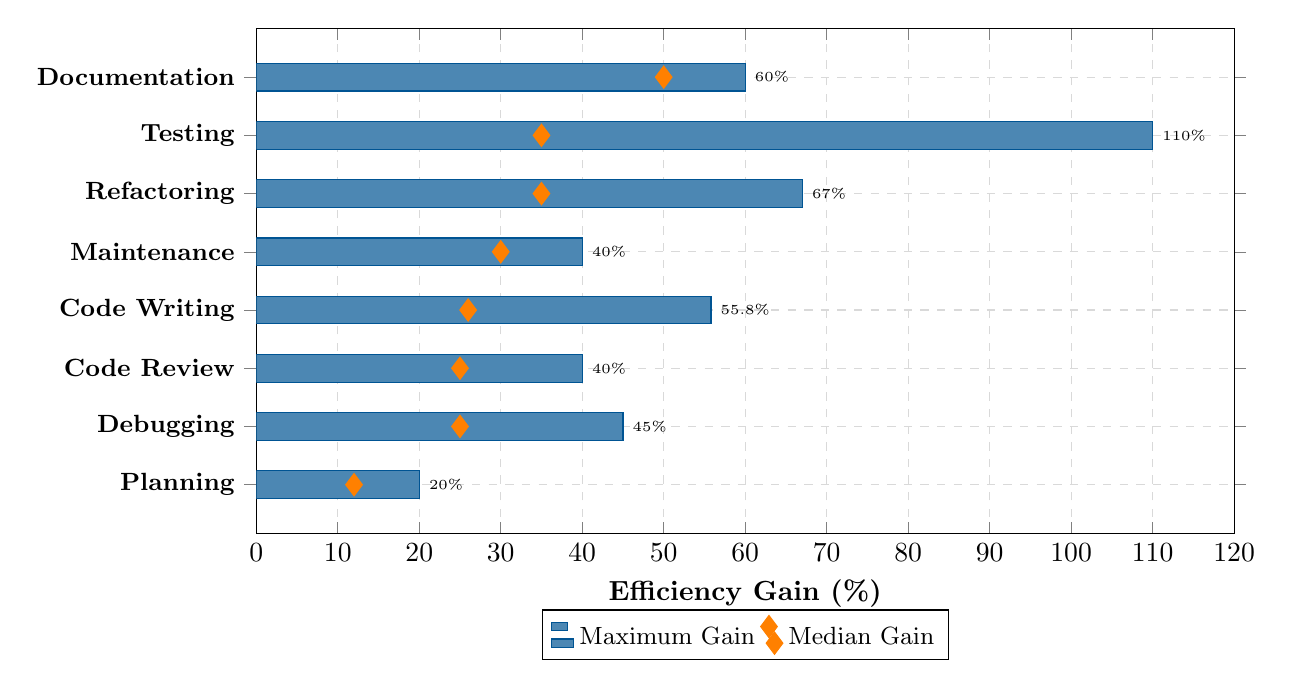
\begin{tikzpicture}
\begin{axis}[
    xbar,
    width=14cm,
    height=8cm,
    xlabel={\textbf{Efficiency Gain (\%)}},
    symbolic y coords={Planning, Debugging, Code Review, Code Writing, Maintenance, Refactoring, Testing, Documentation},
    ytick=data,
    yticklabel style={font=\small\bfseries},
    xmin=0,
    xmax=120,
    bar width=10pt,
    legend style={at={(0.5,-0.15)}, anchor=north, legend columns=2, font=\small},
    legend cell align={left},
    enlarge y limits=0.12,
    grid=major,
    grid style={dashed, gray!30},
    nodes near coords,
    nodes near coords style={font=\tiny, anchor=west},
    point meta=explicit symbolic,
]

% Max values (darker shade)
\addplot[fill=headerblue!70, draw=headerblue] coordinates {
    (20,Planning) [20\%]
    (45,Debugging) [45\%]
    (40,Code Review) [40\%]
    (55.8,Code Writing) [55.8\%]
    (40,Maintenance) [40\%]
    (67,Refactoring) [67\%]
    (110,Testing) [110\%]
    (60,Documentation) [60\%]
};

% Median markers
\addplot[only marks, mark=diamond*, mark size=4pt, fill=orange, draw=orange] coordinates {
    (12,Planning)
    (25,Debugging)
    (25,Code Review)
    (26,Code Writing)
    (30,Maintenance)
    (35,Refactoring)
    (35,Testing)
    (50,Documentation)
};

\legend{Maximum Gain, Median Gain}
\end{axis}
\end{tikzpicture}
\caption{AI Efficiency Gains: Maximum vs. Median by Task Category}
\label{fig:efficiency}
\end{figure}

\vspace{0.3cm}

%% DEVELOPER EXPERIENCE TABLE
\section*{Impact by Experience Level}

\begin{table}[H]
\centering
\renewcommand{\arraystretch}{1.3}
\begin{tabular}{>{\bfseries}l c c c}
\toprule
\rowcolor{headerblue}
\textcolor{white}{\textbf{Task}} & \textcolor{white}{\textbf{Junior (0-2 yrs)}} & \textcolor{white}{\textbf{Mid (3-5 yrs)}} & \textcolor{white}{\textbf{Senior (6+ yrs)}} \\
\midrule
\rowcolor{lightblue}
Code Writing & \textbf{45--55\%} & 30--40\% & 20--30\% \\
Code Review & 25--35\% & 25--35\% & \textbf{30--40\%} \\
\rowcolor{lightblue}
Debugging & \textbf{35--45\%} & 25--35\% & 15--25\% \\
Testing & \textbf{40--50\%} & 35--45\% & 25--35\% \\
\bottomrule
\end{tabular}
\caption{AI Efficiency Gains by Developer Experience Level}
\label{tab:experience}
\end{table}

\vspace{0.5cm}

%% RECOMMENDATIONS
\section*{Recommendations}

\begin{itemize}[leftmargin=*, itemsep=0.3cm]
    \item \textbf{Prioritize AI deployment} for documentation, testing, and code generation (highest ROI)
    \item \textbf{Invest in training} --- full benefits require ~11 weeks of adoption
    \item \textbf{Maintain human oversight} --- AI suggestions require verification
    \item \textbf{Tailor approach by experience} --- junior devs need different support than seniors
\end{itemize}

\vspace{0.5cm}

%% CONCLUSION BOX
\begin{tcolorbox}[colback=lightblue, colframe=headerblue, title=\textbf{Conclusion}]
AI tools deliver \textbf{10--110\% efficiency gains} across software engineering tasks, with median improvements of \textbf{25--50\%}. Documentation and testing show the most consistent benefits. Strategic deployment with proper training and human oversight positions organizations to maximize productivity while maintaining software quality.
\end{tcolorbox}

\vspace{0.5cm}

%% SOURCES
\section*{Key Sources}
\small
\begin{itemize}[leftmargin=*, itemsep=0.1cm]
    \item Peng et al. (2023) --- GitHub Copilot Study, \textit{arXiv}
    \item Meyer et al. (2021) --- Developer Workdays, \textit{IEEE TSE}
    \item McKinsey \& Company (2023) --- Generative AI Productivity Report
    \item DORA Report (2024) --- State of DevOps
    \item Google RCT (2024) --- Internal AI Productivity Study
\end{itemize}

\end{document}
